\documentclass{beamer}

\usepackage{hyperref}
\usepackage{epstopdf} 
\usepackage{graphicx}
\usepackage{amssymb}

\title{Central Trigger Board}
\author{ Update \\ Jonathon Sensenig}
\institute{University of Pennsylvania}
\date{}

% position the logo
%\addtobeamertemplate{frametitle}{}{%
%	\begin{textblock*}{100mm}(\textwidth,-1cm)
%		
\includegraphics[height=1cm,width=1cm,keepaspectratio]{figs/Penn-Shield.png}
%\end{textblock*}}

%Add page number to the foot bar
\expandafter\def\expandafter\insertshorttitle\expandafter{%
	\insertshorttitle\hfill%
	\insertframenumber\,/\,\inserttotalframenumber}

%Use an image as the background
%\usebackgroundtemplate{
%	
\includegraphics[width=\paperwidth,height=\paperheight]{figs/bblue3.pdf}
%

%Add logos to title page only
%\titlegraphic{
\includegraphics[width=1.75cm]{figs/DUNElogo_color.png}\hspace*{2.75cm}~
%	\includegraphics[width=3cm]{figs/shield-logotype-whitebkgd-RGB-4k.png}
%}

\usetheme{Copenhagen}
\setbeamertemplate{navigation symbols}{} %NO nav buttons!

% Color modification
\definecolor{MyBackground}{RGB}{255, 255, 255}
\definecolor{jgrey}{RGB}{121, 147, 179}
\definecolor{jred}{RGB}{181,0,0}
\setbeamercolor{background canvas}{bg=MyBackground}
\setbeamercolor{structure}{fg=jgrey}% to modify  immediately all palettes
\setbeamercolor{title}{fg=black}
\setbeamercolor{title in head/foot}{fg=jred}
\setbeamercolor{author}{bg=black,fg=white}
\setbeamercolor{frametitle}{fg=black}

\begin{document}
	\frame {
		\titlepage
		\hspace{0.2cm}
		
\includegraphics[width=10cm,height=2.25cm]{figs/dune_penn_logo.png}
		
	}	
	
	\frame {
	    \frametitle{Modified PTB  1/2}
	    \framesubtitle{Firmware which is near completion}
	    \begin{figure}
	    	\centering
	    		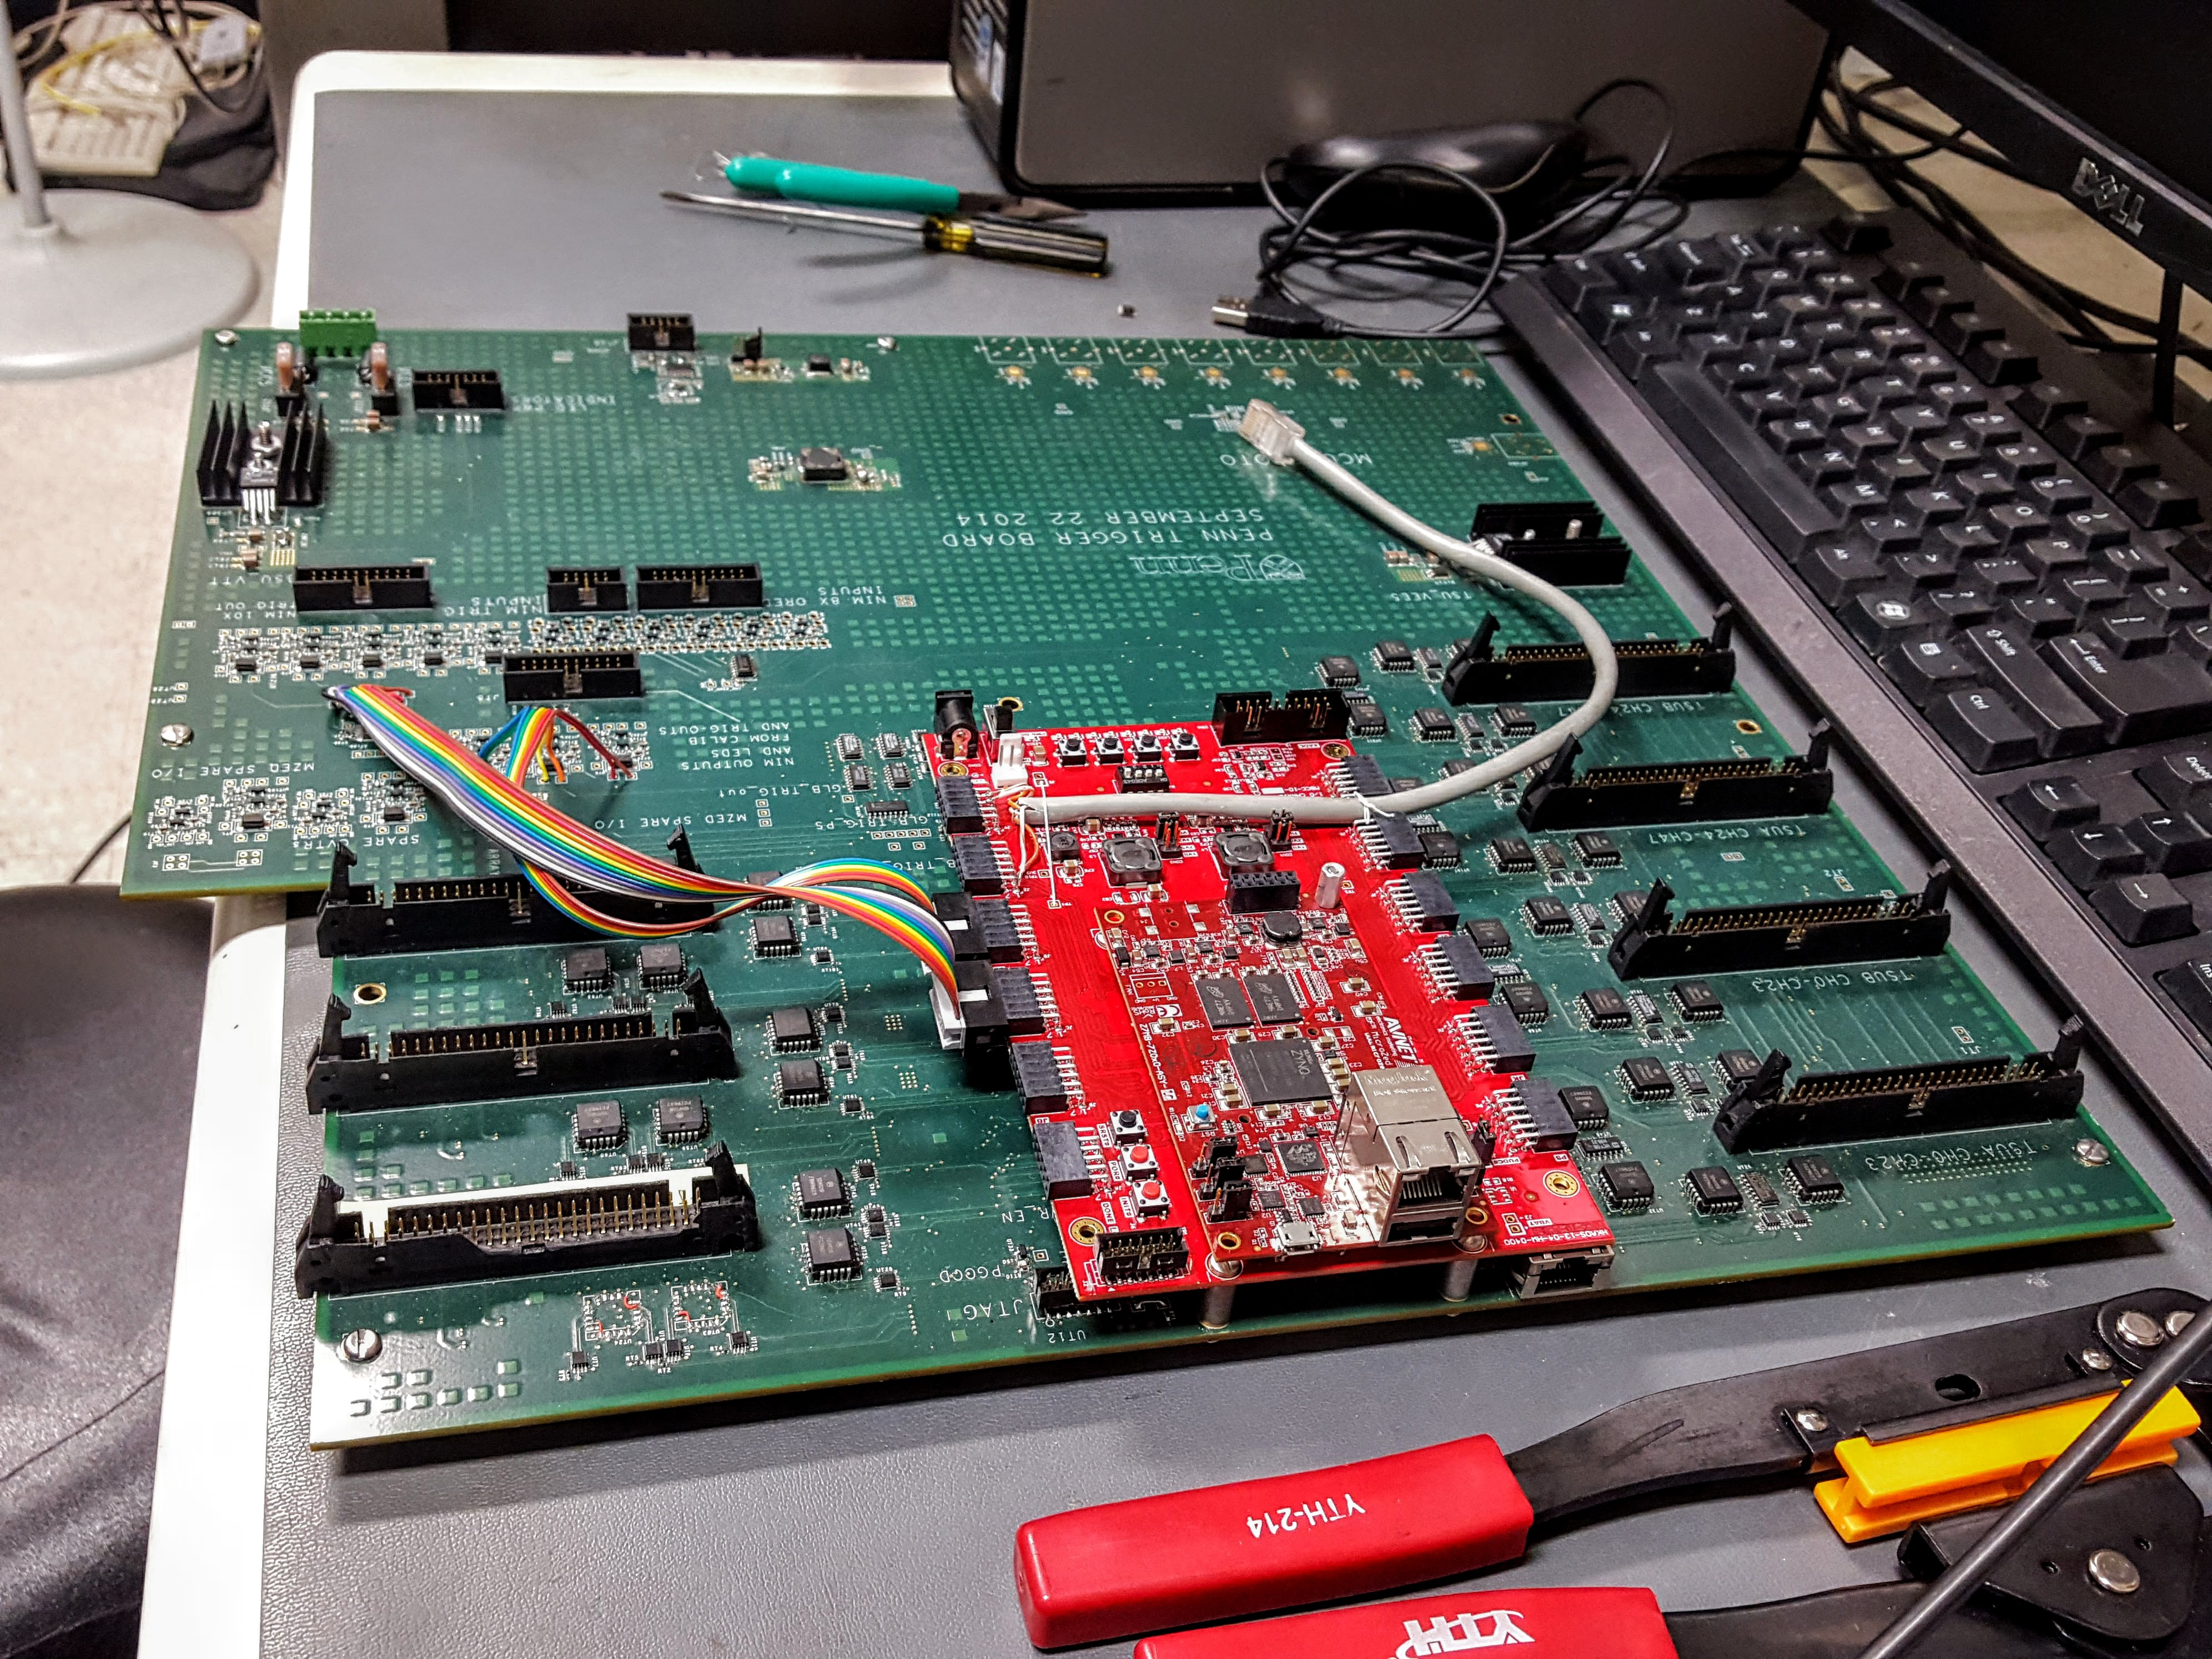
\includegraphics[width=9cm,height=6cm]{figs/ptb_mz.jpg}
	    \end{figure}	
	}
	\frame {
	    \frametitle{Modified PTB  2/2}
	    \framesubtitle{Firmware which is near completion}
		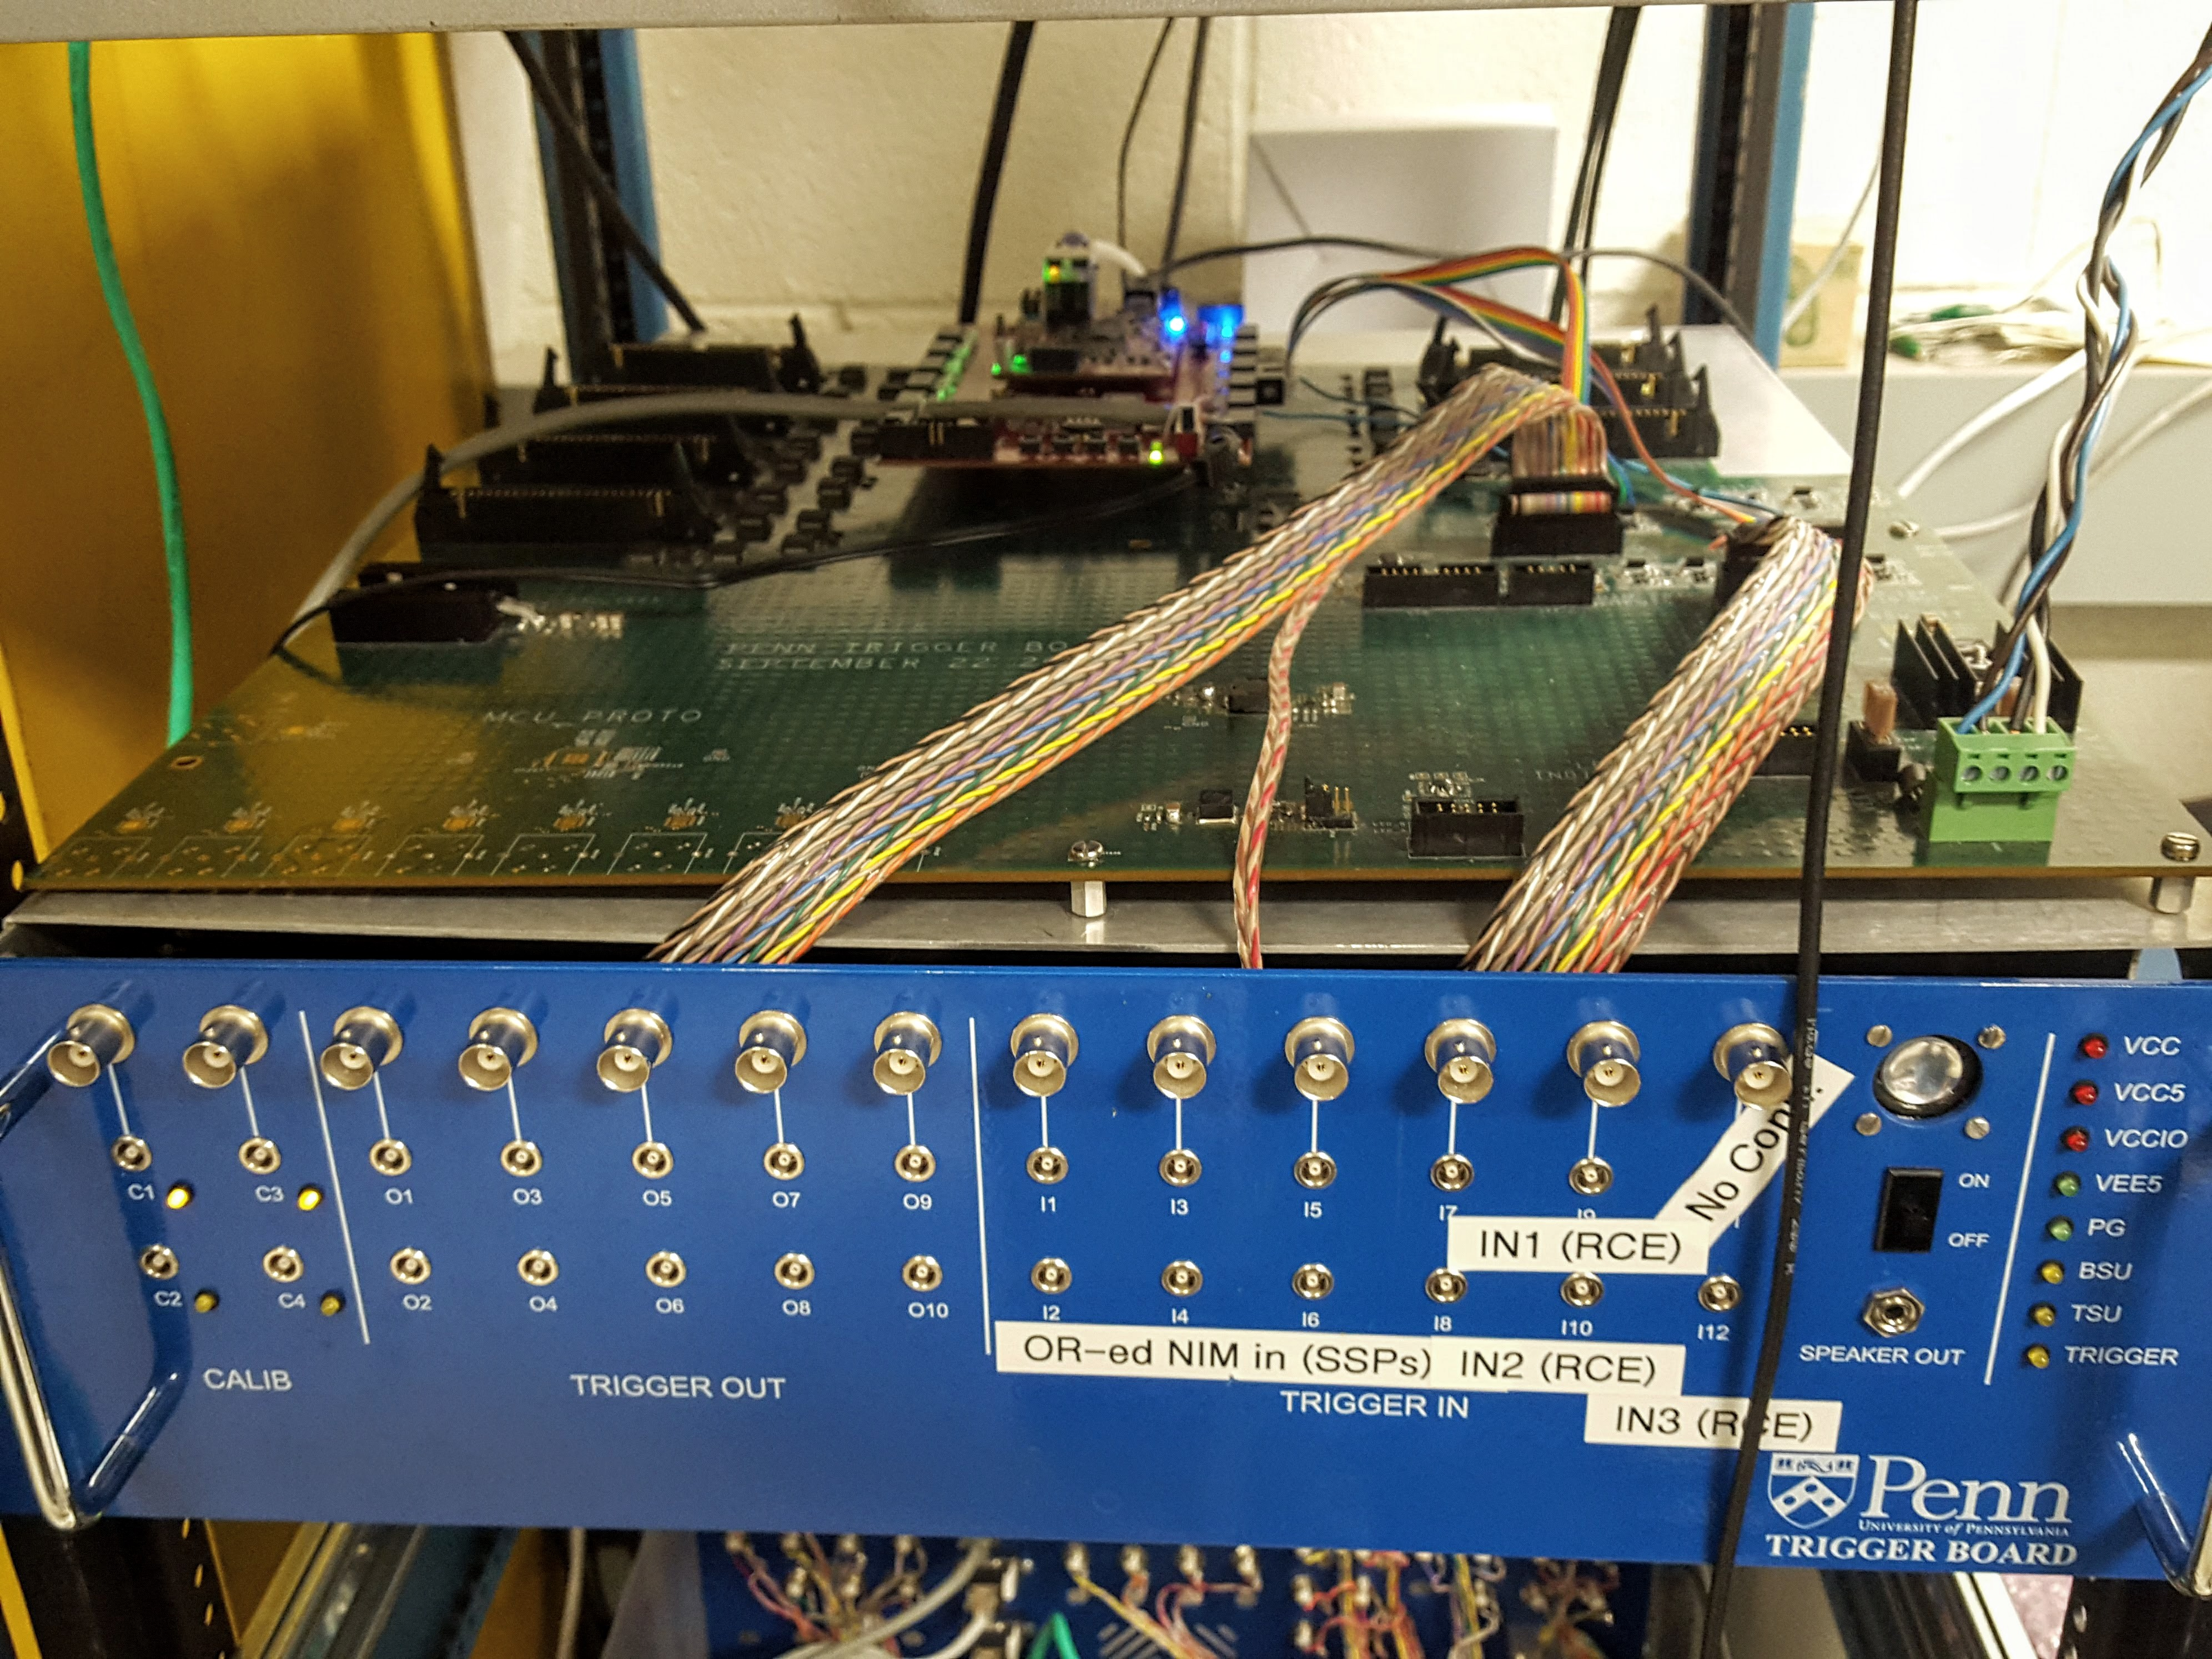
\includegraphics[width=9cm,height=6cm]{figs/ptb_mz_case.jpg}
	}

	\frame {
	\frametitle{Beam Trigger  1/4}
	\framesubtitle{The Beamline as Represented in simulation}
	\begin{figure}
		\centering
		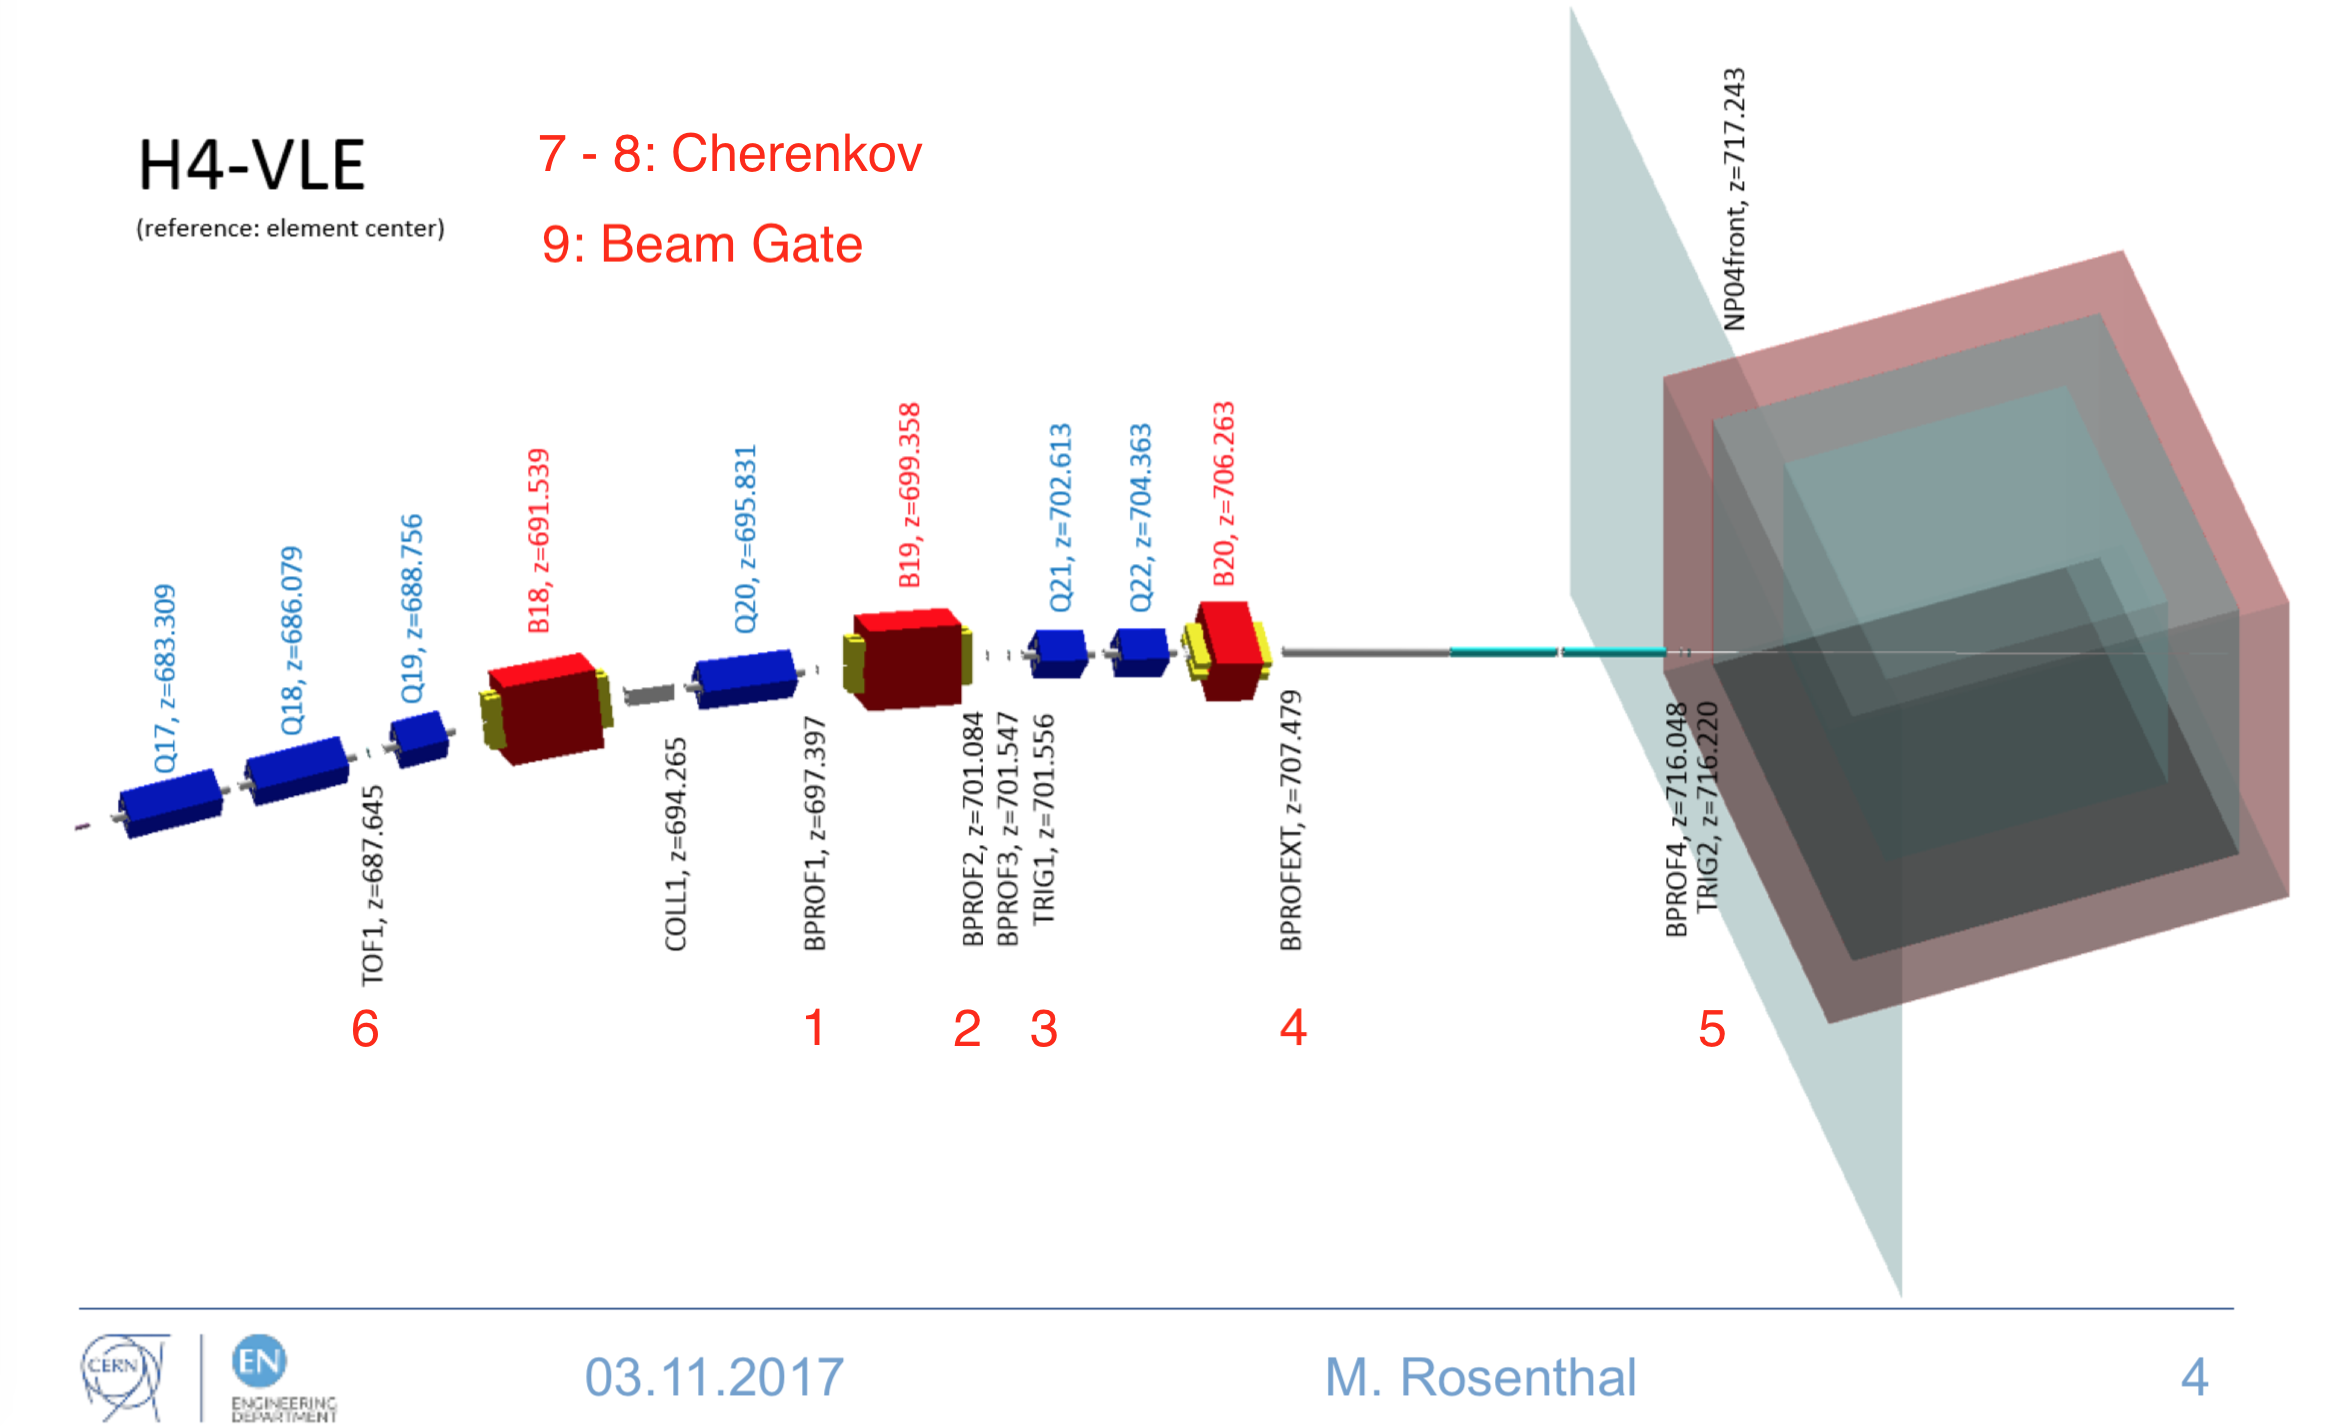
\includegraphics[width=9cm,height=6cm]{figs/h4beam.png}
	\end{figure}
	}

	\frame {
	\frametitle{Beam Trigger  2/4}
	\framesubtitle{Some Questions}
	\begin{itemize}
		\item Is there any reason to trigger if not all fiber trackers fire? Maybe something like $>$3 trackers, low probability of a false trigger and will offset the approx. 6.5\% inefficiency of the trackers.
		\item
	\end{itemize}
	}

	\frame {
	\frametitle{Beam Trigger  3/4}
	\framesubtitle{Jon Paley's Presentation at Collab. Meeting}
	\begin{figure}
		\centering
			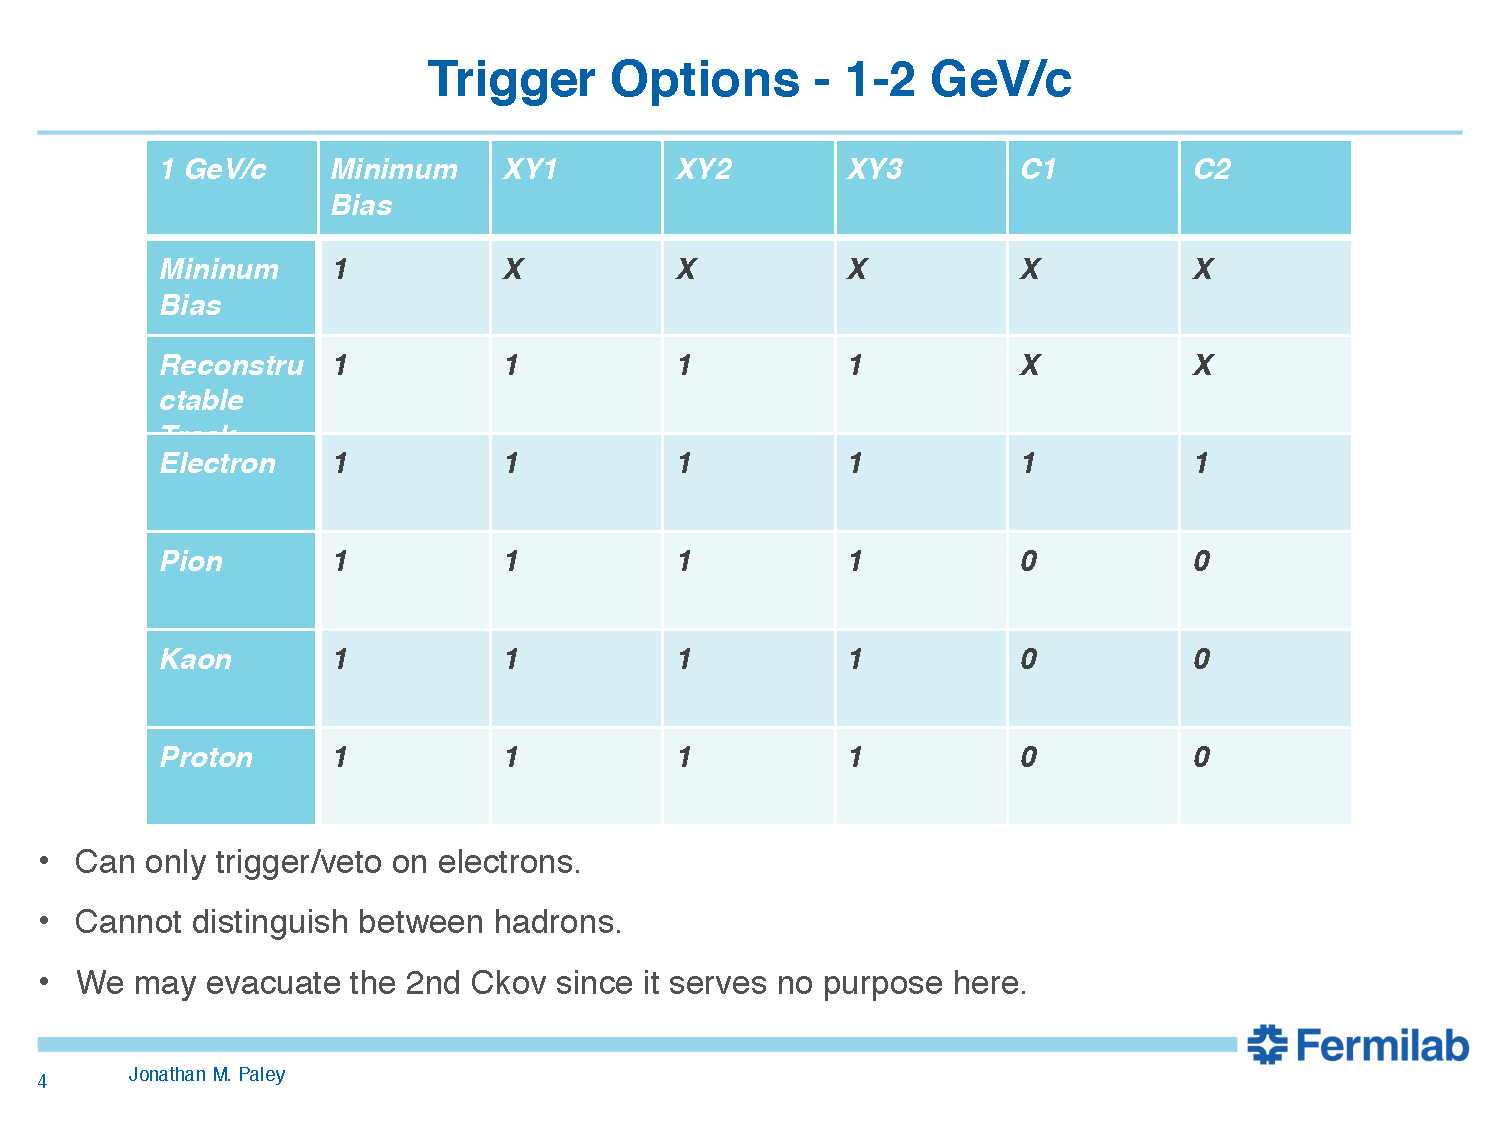
\includegraphics[width=9cm,height=6cm]{figs/2018-01-31_Trigger_Discussion_BI.pdf}
	\end{figure}
	}

	\frame {
	\frametitle{Beam Trigger  4/4}
	\framesubtitle{Beam Triggers Summary}
	\begin{itemize}
		\item Start with all fiber trackers.
		\item Start with 1 - 2 GeV/c triggers since the first run (engineering run) will be with 2GeV/c beam.
	\end{itemize}

	\begin{center}
	\begin{table}[ht]	
		\caption{1-2 GeV/c beam triggers inclusive trigger masks.}
		\centering 
		\begin{tabular}{c c }
			\hline \hline         
			Trigger & $\lbrack$ 8 : 0 $\rbrack$ = $\lbrack$ BG, C2, C1, TOF, BP1-5 $\rbrack$    \\ [0.5ex] 
			\hline 
			No Beam & 0 XX X XXXXX  \\	
			e$^-$ & 1 11 1 11111  \\
			$\pi$/K/p & 1 00 1 11111  \\
			\hline	
		\end{tabular}
		\label{table:bi_trig}	
	\end{table}	
\end{center}
	}
	
	\frame {
	\frametitle{CRT Trigger  1/}
	\framesubtitle{Channel Mapping of CRT Modules  (ref. Camillo M.)}
	\begin{figure}
		\centering
		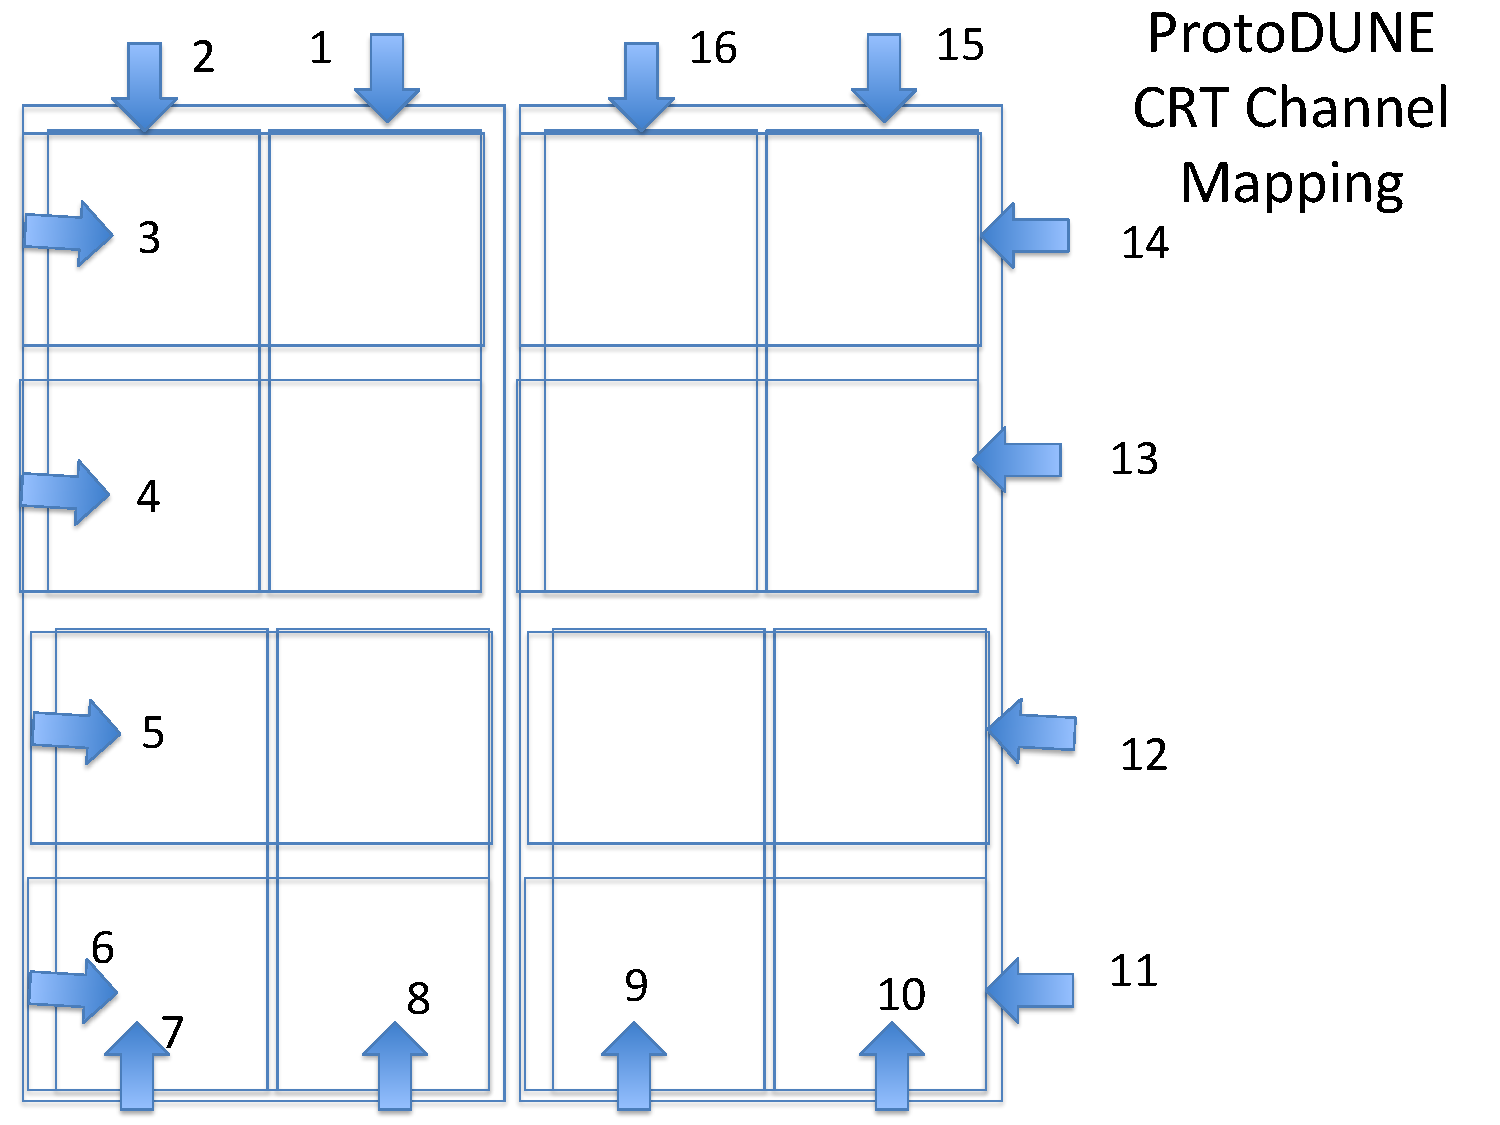
\includegraphics[width=9cm,height=6cm]{figs/crt_mapping.pdf}
	\end{figure}
}
	
\end{document}